\documentclass[listings]{labreport}
\usepackage{amsmath}
\subject{Теория автоматов}
\titleparts{Практическое задание №1}{Вариант 8}
\students{Лабушев Тимофей}

\begin{document}

\maketitlepage

\section*{Цель работы}

Практическое освоение методов взаимного преобразования автоматных моделей Мили и Мура.
Проверка абстрактных автоматов Мили и Мура на эквивалентность.

\section*{Задание}

\begin{enumerate}
\item В соответствии с выбранным номером варианта осуществить преобразование автомата Мили в автомат Мура.
\item Сформировать входное слово необходимой длины. Длина входного слова должна быть минимальна,
  но достаточна для осуществления всех имеющихся в графах автоматов переходов.
\item Используя сформированное входное слово, осуществить проверку исходного и полученного в результате
  преобразования автоматов на эквивалентность. В качестве исходного состояния выбрать состояние $а_1$.
\item Далее осуществить преобразование полученного на предыдущем этапе автомата Мура в автомат Мили.
\item Сформировать входное слово необходимой длины. Длина входного слова должна быть минимальна,
  но достаточна для осуществления всех имеющихся в графах автоматов переходов.
\item Используя сформированное входное слово, осуществить проверку исходного и полученного в результате
  преобразования автоматов на эквивалентность. В качестве исходного состояния выбрать состояние $a_1$.
\end{enumerate}

\section*{Исходный автомат Мили}

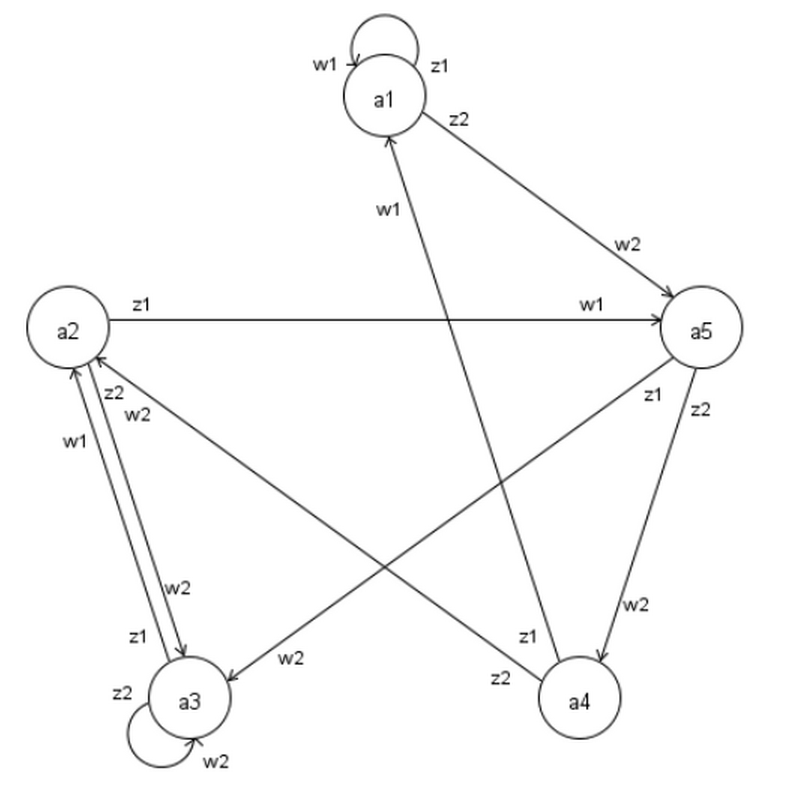
\includegraphics[width=0.6\textwidth]{HW1.png}

\subsection*{Входное слово}

\begin{tabular}{|c|c|c|c|c|c|c|c|c|c|c|c|c|c|}
\hline
$z_1$ & $z_2$ & $z_1$ & $z_2$ & $z_1$ & $z_2$ & $z_1$ & $z_1$ & $z_2$ & $z_1$ & $z_2$ & $z_2$ & $z_2$ & \\\hline

$a_1$ & $a_1$ & $a_5$ & $a_3$ & $a_3$ & $a_2$ & $a_3$ & $a_2$ & $a_5$ & $a_4$ & $a_1$ & $a_5$ & $a_4$ & $a_2$ \\\hline

$w_1$ & $w_2$ & $w_2$ & $w_2$ & $w_1$ & $w_2$ & $w_1$ & $w_1$ & $w_2$ & $w_1$ & $w_2$ & $w_2$ & $w_2$ & \\\hline
\end{tabular}

\newpage

\section*{Преобразование в автомат Мура}

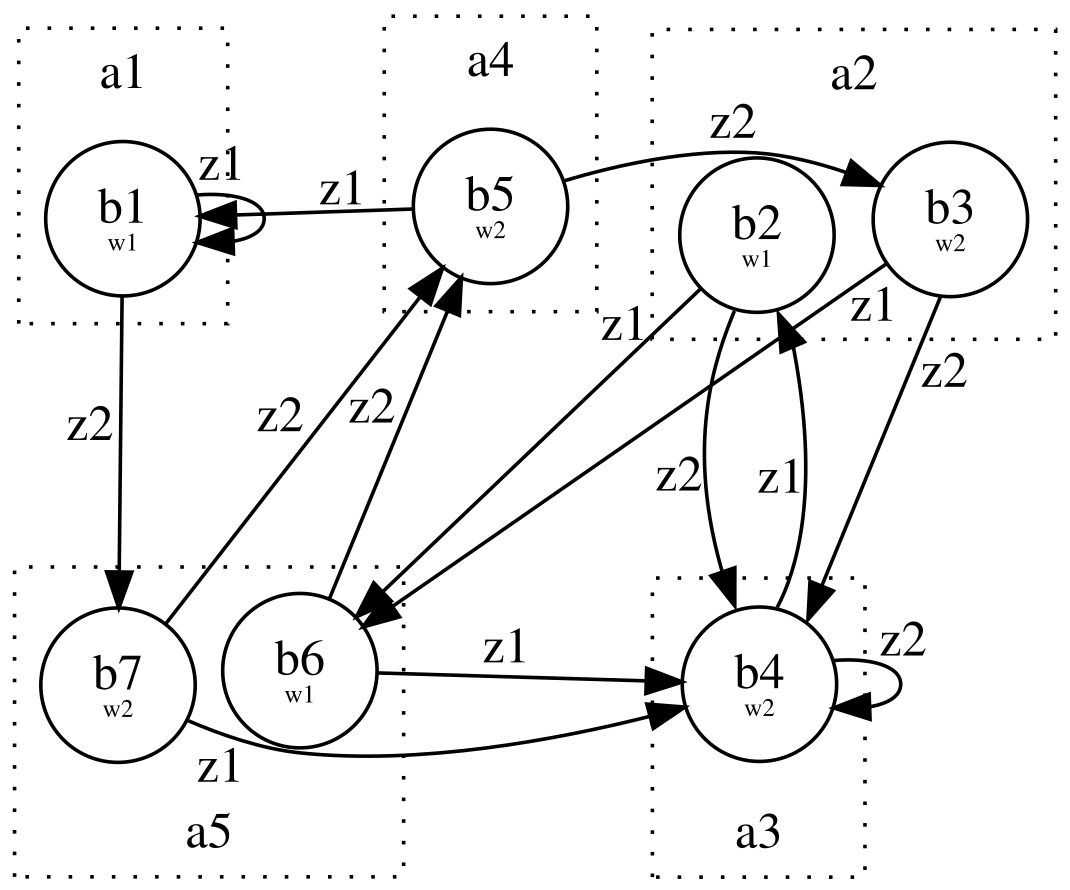
\includegraphics[width=0.5\textwidth]{moore.png}

\subsection*{Проверка на эквивалентность}

\begin{tabular}{|c|c|c|c|c|c|c|c|c|c|c|c|c|c|}
\hline
$z_1$ & $z_2$ & $z_1$ & $z_2$ & $z_1$ & $z_2$ & $z_1$ & $z_1$ & $z_2$ & $z_1$ & $z_2$ & $z_2$ & $z_2$ & \\\hline

$b_1$ & $b_1$ & $b_7$ & $b_4$ & $b_4$ & $b_2$ & $b_4$ & $b_2$ & $b_6$ & $b_5$ & $b_1$ & $b_7$ & $b_5$ & $b_3$ \\\hline

      & $w_1$ & $w_2$ & $w_2$ & $w_2$ & $w_1$ & $w_2$ & $w_1$ & $w_1$ & $w_2$ & $w_1$ & $w_2$ & $w_2$ & $w_2$ \\\hline
\end{tabular}

\section*{Обратное преобразование}

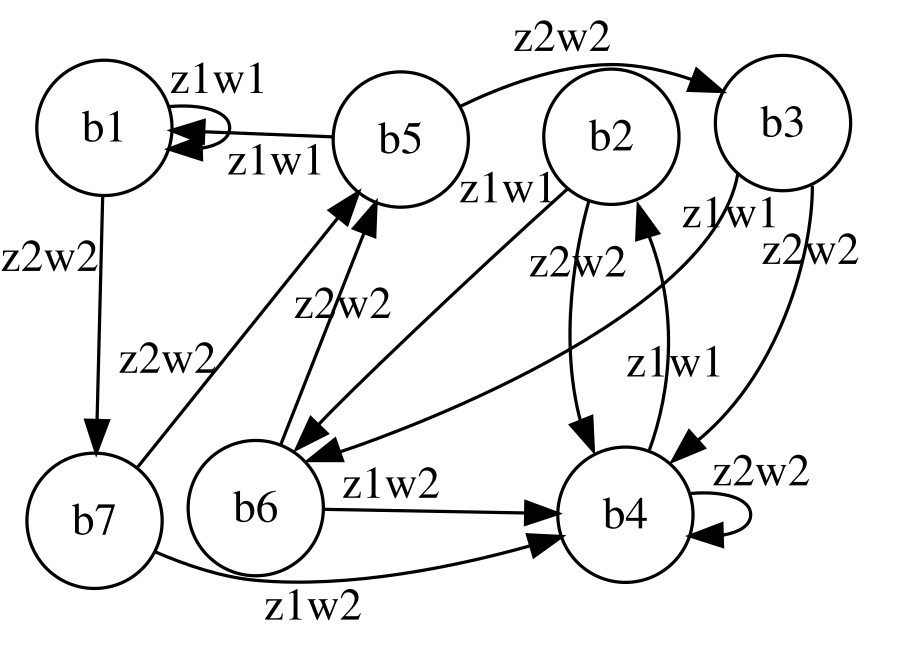
\includegraphics[width=0.5\textwidth]{mealy.png}

\subsection*{Проверка на эквивалентность}

\begin{tabular}{|c|c|c|c|c|c|c|c|c|c|c|c|c|c|}
\hline
$z_1$ & $z_2$ & $z_1$ & $z_2$ & $z_1$ & $z_2$ & $z_1$ & $z_1$ & $z_2$ & $z_1$ & $z_2$ & $z_2$ & $z_2$ & \\\hline

$b_1$ & $b_1$ & $b_7$ & $b_4$ & $b_4$ & $b_2$ & $b_4$ & $b_2$ & $b_6$ & $b_5$ & $b_1$ & $b_7$ & $b_5$ & $b_3$ \\\hline

$w_1$ & $w_2$ & $w_2$ & $w_2$ & $w_1$ & $w_2$ & $w_1$ & $w_1$ & $w_2$ & $w_1$ & $w_2$ & $w_2$ & $w_2$ & \\\hline
\end{tabular}

\end{document}
